\documentclass[14pt, english]{article}
\usepackage[T1]{fontenc}
\usepackage[latin9]{inputenc}
\usepackage{color}
\usepackage{babel}
\usepackage{amsmath}
\usepackage[unicode=true,pdfusetitle,
 bookmarks=true,bookmarksnumbered=false,bookmarksopen=false,
 breaklinks=false,pdfborder={0 0 1},backref=false,colorlinks=true]
 {hyperref}

\makeatletter


\providecommand{\tabularnewline}{\\}

%% guys don't worry about names being in the date section,
%% I did it so that  I could arange it in the order with sub title

\date{Amin Saeidi, Georg Konwisser (Shlomo), and Aaditya Prakash}
\usepackage{graphicx}
\hypersetup{urlcolor=blue}

\makeatother

\begin{document}

\title{Detection of fallacy in natural text}

%% see the comment above for the date section
\author{Final project for CS135: Computational Semantics}

\maketitle

\section{Abstract}

In this project we investigate and build a simple fallacy detection
system in Haskell from natural text. This project implements relation
extraction at level sufficient to allow for conversion of natural
text into logical form. Once the logical form is obtained, we check if the input expression matches the pattern of the fallacy expression. Doing so we accept certain pattern variance appropriate for fallacy detection.
This project is limited to propositional fallacies like 'affirming the disjunct', , only and
does not support other types of fallacies, for example quantification
fallacies and formal syllogistic fallacies. It has been aimed to keep
the parsed input as a free natural text but certain constrained and
structure has been assumed.


\section{Design}

After careful thought and experimenation with several Haskell packages
for First Order Logic conversion ( \href{https://github.com/traeger/fol-solver}{FOL Solver},
\href{https://github.com/marcosccm/enki}{Haskell Inference Engine},
\href{https://github.com/edwinb/Ivor}{Type Theory based theorem prover},
\href{https://github.com/danr/hip}{Haskell Inductive Prover}, \href{http://attempto.ifi.uzh.ch/site/}{University of Zurich's Attempto Project}
and \href{http://homepages.cwi.nl/~jve/courses/12/haskellroad/TOTP.pdf}{Jan van Eijck's TOTP}),
we decided to write our own relation extraction customized for fallacy
proving. There were several reasons for this decision, but few of
them were -

1. Conversion to first order logic, was an overkill for our purposed

2. Most of the libraries we experimented, had their fair share of
issues with compatibility, execution or performance.

3. We wanted to put into practice some of the semantics knowledge
obtained from this class.


\subsection{Converting sentences to logical form}

One of the major challenges of this project was to be able to write
down the provided set of sentences into logical form of simplified
knowledge sets as premises and a conclusion. It was important to track
the modifiers. As mentioned earlier in Abstract, we decided to focus
only on propositional fallacies, thus we did not have to deal with
quantifiers. Following schematic logic was used to convert the text
to logical form.
\item Set the boundaries so that seperate knowledge can be extracted. Replace
the following explicit logic operators -

\begin{enumerate}
\item AND \textquotedbl{}but\textquotedbl{} with keyword \textquotedbl{}and\textquotedbl{}
\textquotedbl{}.\textquotedbl{} with keyword \textquotedbl{}and\textquotedbl{} 
\item IMPLICATION \textquotedbl{}therefore\textquotedbl{} with \textquotedbl{}=>\textquotedbl{}
\textquotedbl{}so\textquotedbl{} with \textquotedbl{}=>\textquotedbl{} 
\end{enumerate}
\item Stem the Sentence as a whole (just normal stemming and not chunking)
(Stemming seperates the sentences with \textquotedbl{}.\textquotedbl{}
as different array elements so that we get different knowledge set
for separate variable) 
\item Tag the sentence (stemming before so that we get the same tags for
the same verb but represented in different format) 
\item Extract the premise and the conclusion part. 
\item Make the premise and the conclusion part, separately into well formed
expression 

\begin{enumerate}
\item Find, NOT in the proposition, extract and apply it to the proposition
as unary operator 
\item Recursively apply OR (Disjunction) and AND (Conjunction) to the list
of propositions variables 
\end{enumerate}
\end{enumerate}

\subsection{Detecting fallacy from logical form}
Once the given set of sentences were converted into logical form,
we employ the following recursive pattern matching algorithm. Matching succeeds if the expression trees only differ at places where
the fallacy expression has leaves (variables). In those cases however the corresponding
part in the input expression tree has to imply the variable in the fallacy expression.
In order to check this implication we evaluate if it is a tautological relation. According to our
exploit of \href{http://en.wikipedia.org/wiki/Tautology_(logic)}{definition of tautology in propositional logic},
tautologies are extended to any logically valid formula.

Since the tree-leaf implication relies on having the same variables in input and fallacy expressions,
we extract the variable set from the input and use it to substitute the variable set in the fallacy expression.

\section{Fallacies implemented}

We have implemented the detection of following propositional fallacies-


\subsection{Affirming the disjunct}

Affirming the disjunct is a type of fallacy which occurs when one
of the logical expression in a set of disjuncts is concluded to be
false in the evidence of another premise. In logical formula, this
is expressed as follows:

\begin{center}
$p\vee q$
\par\end{center}

\begin{center}
$p$
\par\end{center}

\begin{center}
$\implies\neg q$
\par\end{center}

Example of this type of fallacy from Wikipedia: 

\begin{center}
Max is a cat or Max is a mammal.
\par\end{center}

\begin{center}
Max is a cat.
\par\end{center}

\begin{center}
Therefore, Max is not a mammal.
\par\end{center}

Following is the screenshot of parsing the above example in our program.

\begin{figure}[htp]
\makebox[\textwidth][c]{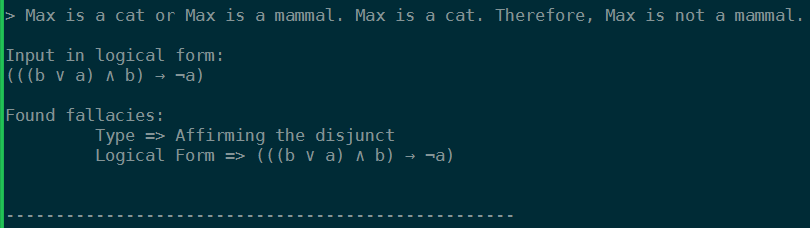
\includegraphics[width=1.3\textwidth]{disjunct}} \caption{Detecting affirming the disjunct} \end{figure}


\subsection{Affirming the consequent}

Affirming the consequent fallacy occurs when given a conditional and
a premise assumes the validity of the consequent. In logical form
this can be expressed as follows:

\begin{center}
$p\to q$
\par\end{center}

\begin{center}
$q$
\par\end{center}

\begin{center}
$\implies p$
\par\end{center}

Example of this type of fallacy from Wikipedia: 

\begin{center}
If Bill Gates owns Fort Knox, then he is rich.
\par\end{center}

\begin{center}
Bill Gates is rich.
\par\end{center}

\begin{center}
Therefore, Bill Gates owns Fort Knox.
\par\end{center}

Following is the screensho of parsing the above example (without anaphora
resolution) in our program:

\begin{figure}[htp]
\makebox[\textwidth][c]{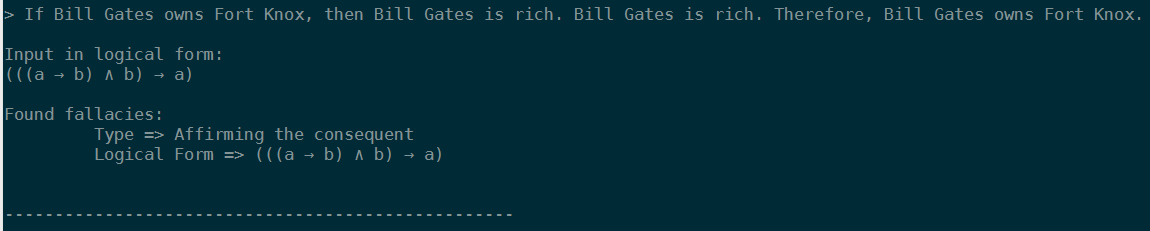
\includegraphics[width=1.3\textwidth]{consequent}} \caption{Detecting affirming the consequent} \end{figure}


\subsection{Denying the antecedent}

Denying the antecedent is similar in strucutre to affirming the consequent
but different in intepretation. In denying the antecedent, given a
conditional and invalidity of the antecedent, fallacy is to assume
invalidity of consequent. In logical form this can be expressed as
follows:

\begin{center}
$p\to q$
\par\end{center}

\begin{center}
$\neg p$
\par\end{center}

\begin{center}
$\implies\neg q$
\par\end{center}

Example of this type of fallacy from Wikipedia: 

\begin{center}
If Queen Elizabeth is an American citizen, then she is a human being.
\par\end{center}

\begin{center}
Queen Elizabeth is not an American citizen.
\par\end{center}

\begin{center}
Therefore, Queen Elizabeth is not a human being.
\par\end{center}

Following is the screensho of parsing the above example (without anaphora
resolution) in our program:

\begin{figure}[htp]
\makebox[\textwidth][c]{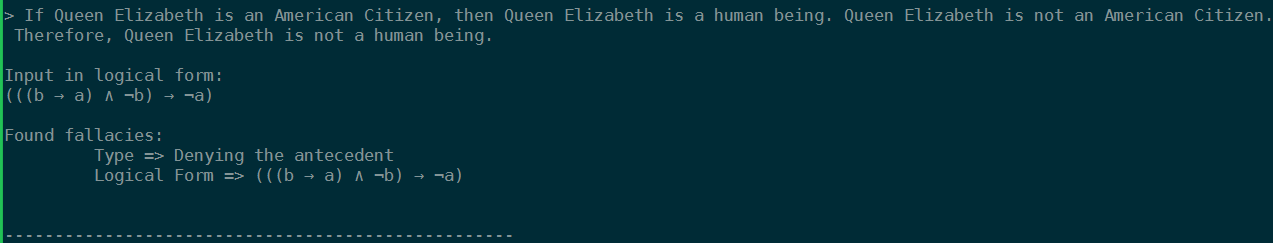
\includegraphics[width=1.4\textwidth]{antecedent}} \caption{Detecting denying the antecedent} \end{figure}


\section{Code}

A brief description of each of the haskell file has been provided
below. For detailed analsis, kindly refer to the function headers
and inline comments in those code files. 
\medskip{}


\begin{tabular}{rl}
Source & Description\tabularnewline
\hline 
Main.hs & Serves as the entry point of the application. See README.md{*} for
usage.\tabularnewline
Detector.hs & Checks for fallacy, when provided with expression in propositional
logic.\tabularnewline
LogicalShortcuts.hs & Makes shortcuts for the logical operations in propostional logic.\tabularnewline
Tests.hs & Includes the unit tests for different modules of the application.\tabularnewline
TextToLogical.hs & Converts the given natural text into propositional logic form for
the fallacy.\tabularnewline
\end{tabular}

\medskip{}


{*}On the root folder of the submission, README.md file has been provided
with detailed instruction on running the modules and the unit tests.

\section{Challenges}
We faced several challenges, some technical and some conceptual while building this application. One of the challenges during parsing was to be able to separate the knowledge set when a sentence had multiple conjunctions and disjunctions. Natural text is enlarge has ambiguities and we tried to limit the scope of the project so that we could make a working prototype. While detecting the fallacies, we encountered several scenarios in which only a subset of the given expression was a fallacy, thus we had to deal with search space to detect fallacies.  

\section{Further Work}

We see this as start of the project and envision this to extend for
all kinds of fallacies and more sophisticated sentence structures. We 
also plan to implement anaphora resolution, so that simple pronouns
in the given premise may be bound to same knowledge set. Another immediate
extension would be to extend this from propositional logic to first
order logic so that quantification fallacies like existential fallacy
could be detected. We also aim to make the parser work with implicit
conclusion rather than explicit conclusion with verbal cues.
 
\medskip{}
We plan to build a web interface that allows user to enter arbitrary sentences and find the fallacy. This can also be used as educational tool for the introductory logic classes.

\end{document}
